\chapter[Radar]{Relatório Radar}
\begin{enumerate}

\item \textbf{Descrição}

Um radar mede uma distância, velocidade ou ângulo de objetos através da utilização de ondas de rádio. O radar emite ondas de rádio que são refletidas por objetos e depois capta e processa essas ondas refletidas para obtenção das informações desejadas tendo como base as propriedades das ondas eletromagnéticas.

As principais propriedades dessas ondas são:

\begin{itemize}
  \item A energia normalmente viaja em uma linha reta a uma velocidade constante;
  \item Energia eletromagnética viaja aproximadamente à velocidade da luz;
  \item Essas ondas são refletidas.
\end{itemize}

\begin{figure}[h]
  \centering
  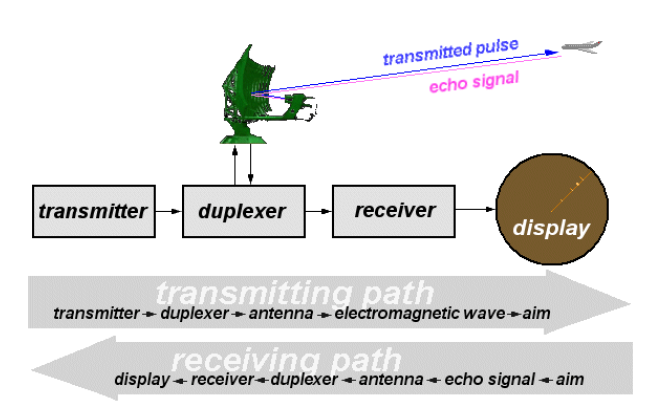
\includegraphics[width=400px, scale=1]{figuras/funcionamento_radar}
  \caption{Esquemático do funcionamento do radar}
\label{fig:funcionamento_radar}
\end{figure}

\item \textbf{Funcionamento}

Os radares funcionam com a emissão de pulsos (transmitted pulses) para posterior detecção dos pulsos refletidos
(echo pulses), isso serve para uma sincronização necessária para a medição de distâncias, já que os pulsos
 são emitidos sequencialmente após um período de tempo (PRT) e os pulsos possuem
  uma largura determinada.

\begin{figure}[h]
  \centering
  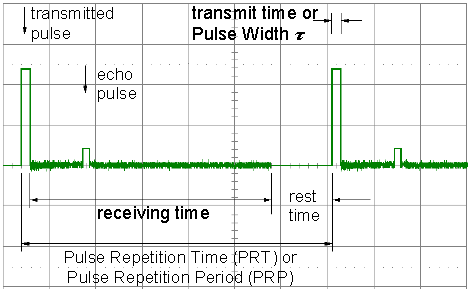
\includegraphics[width=400px, scale=1]{figuras/emissao_pulsos_radar}
  \caption{Gráfico representativo da emissão de pulsos por um radar}
\label{fig:emissao_pulsos_radar}
\end{figure}

A distância entre o radar e o objeto que se quer saber a distância é dada por essa simples equação:

$ R = \displaystyle\frac{Tdelay * C0}{2}$

Onde:

	R: é a distância até o objeto.

	tdelay: é o tempo para o sinal viajar e retornar.

	c0: é a velocidade da luz.

  E as equações para as distâncias máximas e mínimas que um radar pode detectar sem
  causar ambiguidade, sendo trecovery o tempo de recuperação do equipameto
   utilizado, são:


$ Rmax = \frac{(PRT - t) * C0}{2}$

$ Rmin = \frac{(t + Trecovery) * C0}{2}$

\item \textbf{Equação teórica do radar:}

$p_{r} = \frac{\pi ^{2}p_{t}g^{2}\theta h |K|^{2}l2}{1024ln(2)\lambda ^{2}\gamma ^{2}}$

Onde:

Pt = potência transmitida pelo radar (watts)
Pr = potência recebida pelo radar (watts)
g = ganho da antena.
$ \theta $ = tamanho do raio horizontal (radians)
$\varphi$ = tamanho do raio vertical (radians)
h = tamanho do pulso (m)
|K|2 = constante dielétrica.
l = fator de atenuação do raio do radar.
$\lambda$ = comprimento de onda do pulso (m)
r = distância do alvo.
z = fator de refletividade do radar (mm6/m3)

\item \textbf{Especificações do Radar}

\begin{enumerate}
  \item Solução Fechada

  Radar ARS-30X da Continental.
  \begin{enumerate}
    \item Performance:
      \begin{table}[]
      \centering
      \label{habitacao}
      \begin{tabular}{|l|l|p{5cm}|}
      \hline
      Performance de medição &  & Para alvos naturais (não reflexivos)\\ \hline
      Faixa de distância       &  & 0,25 até 200 m campo distante, 0,25 até 60 m distâncias próximas \\ \hline
      Resolução da medição da distância & & 2 m ou > 5,5 km/h (habilidade de separar alvos de objetos)\\ \hline
      Precisão da medição da distância & & A,25 m ou 1,5\%@>1 m\\ \hline
      Aumento do ângulo de azimute & (campo de visão) & -8,5º até +8,5º campo distante -28º até +28º distâncias próximas\\ \hline
      Aumento do ângulo de elevação & (campo de visão) & 4,3º à 6 dBm\\ \hline
      Resolução da medição do ângulo & & 1º campo distante, 4º distâncias próximas\\ \hline
      Precisão da medição do ângulo & & 0,1º campo distante, 1º até 2º para distâncias próximas\\ \hline
      Faixa de velocidade & & -88 km/h até +265 km/h (- se distanciando ... + se aproximando)\\ \hline
      Resolução da velocidade & & 2,76 km/h campo distante, 5,52 km/h distâncias próximas\\ \hline
      Precisão da velocidade & & 0,5 km/h campo distante, 1,0 km/h distâncias próximas\\ \hline
      Tempo de ciclo & & 66 ms\\ \hline
      Tempo de reconhecimento de bloqueio & & <= 60 s\\ \hline
      Quantidade da antena & & 17 campo distante, 15 distâncias próximas\\
      \hline
      \end{tabular}
      \caption{Performance}
      \end{table}

    \item Condições de Operação:

      \begin{table}[]
      \centering
      \label{habitacao}
      \begin{tabular}{|p{5cm}|l|p{5cm}|}
      \hline
      Banda de frequência de operação do radar &  & 76...77 GHz\\ \hline
      Capacidade de transmissão & mediano & < 10 mW\\ \hline
      Rede elétrica de alimentação & à 12 V DC / 24 V DC & 
+8,0 V ... 27 V DC / +8,0 V ... 34 V DC\\ \hline
      Consumo de energia & à 12 V DC / 24 V DC & 7 W à 14 V DC / 7 W à 28 V DC\\ \hline
      Consumo de energia & com aquecimento & Máximo 35 W à 14 V / máximo 63 W à 28 V\\ \hline
      Sistema de alta voltagem & à 12 V DC & Até 27 V DC sem limite de tempo\\ \hline
      Sistema de alta voltagem & à 24 V DC & Até 36 V DC 5 min até 50 V DC 2 min\\ \hline
      Temperatura de operação/armazenamento & & -40 ºC até +85 ºC / -50 ºC até +105 ºC\\ \hline
      Choque & mecânico & 50 g\\ \hline
      Vibração & mecânico & 20 m/s2 @ 10 Hz / 0,14 m/s2 @ 1000 Hz\\ \hline
      Taxa de proteção & & IP 6k 9k (poeira, limpeza de alta pressão)
IP 6k7 (10 cm abaixo da água)
Testado por choque com água e gelo, resistente à nevoeiro salinizado, mistura de gás EM 60068-2-60\\
      \hline
      \end{tabular}
      \caption{Operação}
      \end{table}

    \item Habitação:
      \begin{table}[]
      \centering
      \label{habitacao}
      \begin{tabular}{|l|l|l|}
      \hline
      Dimensões/peso & W*H*D (mm) / massa & $ 120*90*46 / < 500 g $\\ \hline
      Material       & Frente da habitação / parte de trás & Resina de vidro Epoxy / alumínio \\
      \hline
      \end{tabular}
      \caption{Habitação}
      \end{table}
    
  \end{enumerate}
\end{enumerate}


\item \textbf{Solução Aberta}
Soluções abertas, a serem definidas pelos equipamentos utilizados em sua produção caso se deseje montar um da
Figura \ref{fig:esquematico_radar}.
\begin{figure}[h]
  \centering
  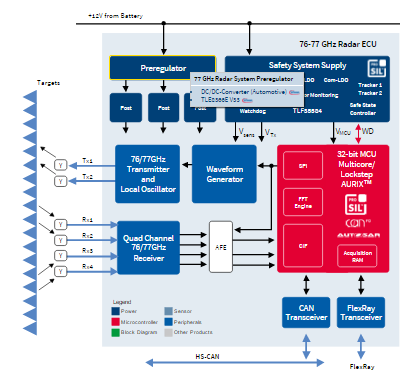
\includegraphics[width=400px, scale=1]{figuras/esquematico_radar}
  \caption{Esquemático dos componentes de um radar}
\label{fig:esquematico_radar}
\end{figure}
\end{enumerate}
